% documento de exemplo modificado a partir do modelo original para teses e dissertações do 
% Programa de Pós-Graduaçãoe em Ciência da Comptuação da UFMG - PPGCC-UFMG, onde as teses 
% foram substituídas por TCCs
\documentclass[proposal]{ppgccufmg} % utilizem 'tcc' para a monografia final ou 'proposal' para projeto de TCC

\usepackage[T1]{fontenc}
\usepackage[utf8]{inputenc}
\usepackage[brazil]{babel}      % se o documento for em português, OU
\usepackage[latin1]{inputenc}
\usepackage[opções]{subfigure}
\usepackage{graphicx}
\usepackage[a4paper,
  portuguese,
  bookmarks=true,
  bookmarksnumbered=true,
  linktocpage,
  colorlinks,
  citecolor=black,
  urlcolor=blue,
  linkcolor=blue,
  filecolor=black,
  ]{hyperref}
\usepackage[square]{natbib}


\begin{document}

% O comando a seguir, \ppgccufmg, provê todas as informações relevantes para a
% classe ppgccufmg. Por favor, consulte a documentação para a descrição de
% cada chave.

% Um exemplo para documentos em português é apresentado a seguir:
\ppgccufmg{
  title={Seleção de características para prognostico de falhas em sistemas dinâmicos},
  authorrev={Borges de Matos, Paulo Augusto},
  cutter={D1234p},   % dados que futuramente serão utilizados pela biblioteca
  cdu={519.6*82.10}, % dados que futuramente serão utilizados pela biblioteca
  university={Instituto Federal do Norte de Minas Gerais},
  campus={Montes Claros},
  coursetype = {Bacharelado},
  course={Ciência da Computação},
  address={Montes Claros},
  date={2019-04},
  keywords={Visão Computacional, Redes, Sabotagens},
  advisor={Luciana Cosme Balieiro},
%  approval={img/approvalsheet.eps},
  abstract={Resumo}{resumo},
  abstract=[english]{Abstract}{abstract},
  dedication={dedicatoria},
  ack={agradecimentos},
  epigraphtext={A verdade é o contrário da mentira, \\
    e a mentira é o oposto da verdade.}{Autor desconhecido},
}

% caso tenha a necessidade de incluir algumas configurações adicionais...
% Os três comandos seguintes são apenas para gerar texto para ocupar espaço nas
% páginas.
\newcommand{\dummytxta}{%
Lorem ipsum dolor sit amet, consectetur adipisicing elit, sed do
eiusmod tempor incididunt ut labore et dolore magna aliqua. Ut enim ad
minim veniam, quis nostrud exercitation ullamco laboris nisi ut
aliquip ex ea commodo consequat. Duis aute irure dolor in
reprehenderit in voluptate velit esse cillum dolore eu fugiat nulla
pariatur. Excepteur sint occaecat cupidatat non proident, sunt in
culpa qui officia deserunt mollit anim id est laborum.\par
}

\newcommand{\dummytxtb}{%
Sed ut perspiciatis unde omnis iste natus error sit voluptatem accusantium
doloremque laudantium, totam rem aperiam, eaque ipsa quae ab illo inventore
veritatis et quasi architecto beatae vitae dicta sunt explicabo. Nemo enim
ipsam voluptatem quia voluptas sit aspernatur aut odit aut fugit, sed quia
consequuntur magni dolores eos qui ratione voluptatem sequi nesciunt. Neque
porro quisquam est, qui dolorem ipsum quia dolor sit amet, consectetur,
adipisci velit, sed quia non numquam eius modi tempora incidunt ut labore et
dolore magnam aliquam quaerat voluptatem. Ut enim ad minima veniam, quis
nostrum exercitationem ullam corporis suscipit laboriosam, nisi ut aliquid ex
ea commodi consequatur? Quis autem vel eum iure reprehenderit qui in ea
voluptate velit esse quam nihil molestiae consequatur, vel illum qui dolorem
eum fugiat quo voluptas nulla pariatur?\par
}

\newcommand{\dummytxtc}{%
At vero eos et accusamus et iusto odio dignissimos ducimus qui blanditiis
praesentium voluptatum deleniti atque corrupti quos dolores et quas molestias
excepturi sint occaecati cupiditate non provident, similique sunt in culpa qui
officia deserunt mollitia animi, id est laborum et dolorum fuga. Et harum
quidem rerum facilis est et expedita distinctio. Nam libero tempore, cum soluta
nobis est eligendi optio cumque nihil impedit quo minus id quod maxime placeat
facere possimus, omnis voluptas assumenda est, omnis dolor
repellendus. Temporibus autem quibusdam et aut officiis debitis aut rerum
necessitatibus saepe eveniet ut et voluptates repudiandae sint et molestiae non
recusandae. Itaque earum rerum hic tenetur a sapiente delectus, ut aut
reiciendis voluptatibus maiores alias consequatur aut perferendis doloribus
asperiores repellat.\par
}

\newcommand{\dummytxt}{\dummytxta\dummytxtb\dummytxtc}

% Inclua cada capítulo em um arquivo separado para melhorar a organização
\chapter{Introdução}
\begin{comment}
Segundo \cite{horn86robot}, todo triângulo equilátero tem os lados iguais. Já
segundo \cite{shashua97photometric}, todo quadrado também tem. \cite{Li2009}

Veja que o pacote \verb|natbib| permite uma série de formas diferentes para
fazer referências bibliográficas. O comando padrão, \verb|\cite|, realiza a
citação comum vista no parágrafo anterior. Outros comandos permitem, por
exemplo, citar somente o autor --- por exemplo, citar o trabalho de
\citeauthor{samaras99coupled} --- ou colocar automaticamente a citação entre
parênteses \citep{hougen93estimation, sato99illumination2, sato99illumination1,
sato01stability}. Os comandos usados foram, respectivamente, \verb|\citeauthor|
e \verb|\citep|. Veja a documentação do \verb|natbib| na Internet para conhecer
outros comandos e exemplos de uso. 

Citações aleatórias para fazer com que as referências bibliográficas ocupem
mais de uma página: \cite{bichsel92simple, dror01statistics, guisser92new}.
\end{comment}

Dado que um banco de dados, temos que um conjunto muito grande de características presentes nele, muitas vezes essas características não são relevantes. A seleção de características é necessário se obter previamente um conjunto de características, através da análise constante de tais características será possível fazer as análises e a predição do estado da máquina.

\section{Motivação e Relevância}

\dummytxtb\dummytxta

\section{Objetivos}

\dummytxtb\dummytxta

\subsection{Objetivos específicos}


\dummytxtc\dummytxtb

\section{Estrutura do Trabalho}

\dummytxta\dummytxtc

\subsubsection{Descendo mais um nível}

\dummytxtb\dummytxta

\chapter{Conceitos Básicos}
\section{Prognóstico}
O Prognostico é usado para predizer a vida útil restante (RUL) de um sistema. A RUL é utilizada para poder dizer ate quando um sistema irá funcionar corretamente, e além disso informar possíveis atualizações que podem ser feitas. A RUL pode ser obtida a partir dos dados obtidos através de sensores em um sistema, esses podem ser sensoriais, características ou até mesmo um resíduo de uma previsão do modelo. O monitoramento do sistema, geralmente uma máquina, é feita de forma constante e ininterrupta, de forma que os dados possam ser obtidos a todo momento, os dados coletados e analisados constantemente de forma que a todo momento a RUL possa ser atualizada \cite{liao2014discovering}.

O prognostico se tornar muito eficaz quando feito corretamente, através dele é possível que uma indústria quando nos referimos a maquinas, exemplo a máquina CNC, ele poderá nos dizer se a maquina está trabalhando corretamente, evitando futuros acidentes e perdas de material, dessa forma, o prognostico de falhas poderá dizer até quando uma máquina funcionara antes de apresentar defeitos ou parar de funcionar, sendo assim ajudando na tomada de decisão de futuras manutenções ou substituições de peças.

A máquina CNC muito utilizada na indústria, é utilizada para o corte de peças com alta precisão e alta produtividade \cite{inacioprognostico}. A máquina CNC através de uma programação é capaz de cortar várias peças de metal em grande velocidade e de forma uniforme. A deia do prognóstico em tais máquina é manter essa uniformidade de forma a evitar o prejuízo da empresa. Na figura 2.1 podemos ver como é uma máquina CNC e como sensores para captação de dados seriam.



\begin{figure}[h]
    \centering
    %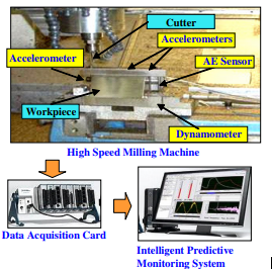
\includegraphics{img/CNC}
    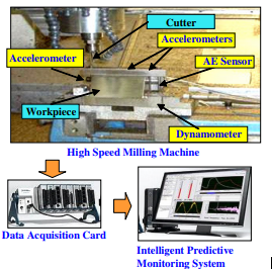
\includegraphics[scale=1]{img/CNC}
    \caption{Monitoramento das condições da ferramenta no processo de fresamento em alta velocidade}
\end{figure}

\begin{figure}[h]
  \centering
  \mbox{%
    \subfigure[Desgaste da ferramenta (cutter1).]{\label{avr-prgmem}%
      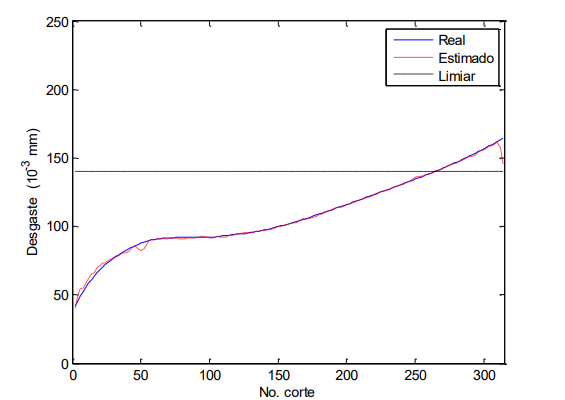
\includegraphics[scale=.4]{img/d1}}\qquad
    \subfigure[RUL da ferramenta (cutter1).]{\label{avr-datamem}%
      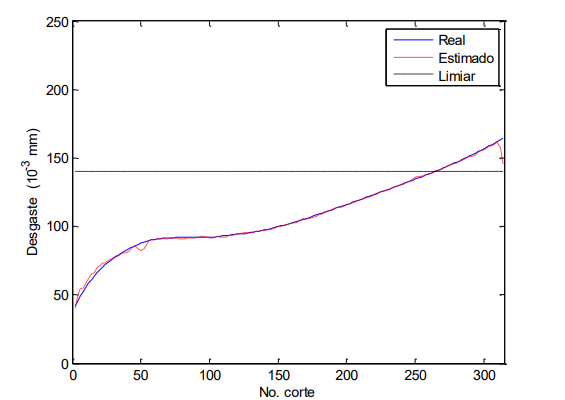
\includegraphics[scale=.4]{img/d1}}
    }
  \caption{Analise Cutter 1 \cite{inacioprognostico}}
  \label{avr-memmap}
\end{figure}


Nas figuras 2.2(a), 2.3(a), 2.4(a) podemos ver a comparação entre o desgaste real e o desgaste obtido pelo Prognostico de Falhas.


\begin{figure}[h]
  \centering
  \mbox{%
    \subfigure[Desgaste da ferramenta (cutter4).]{\label{avr-prgmem}%
      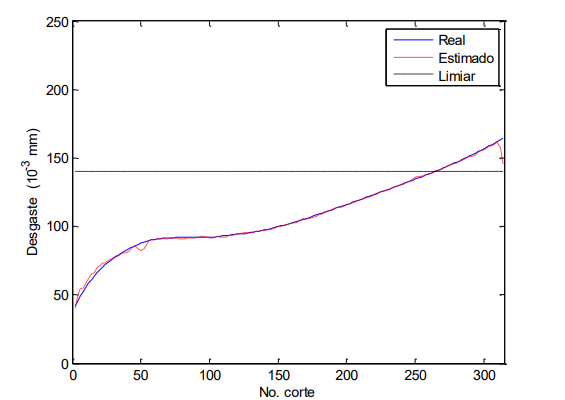
\includegraphics[scale=.4]{img/d1}}\qquad
    \subfigure[RUL da ferramenta (cutter4).]{\label{avr-datamem}%
      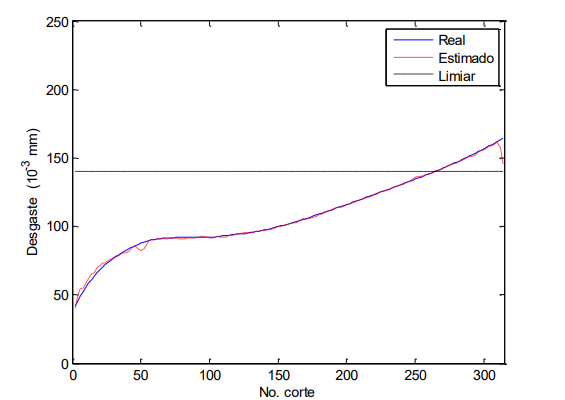
\includegraphics[scale=.4]{img/d1}}
    }
  \caption{Analise Cutter 4 \cite{inacioprognostico}}
  \label{avr-memmap}
\end{figure}

\begin{figure}[h]
  \centering
  \mbox{%
    \subfigure[Desgaste da ferramenta (cutter6).]{\label{avr-prgmem}%
      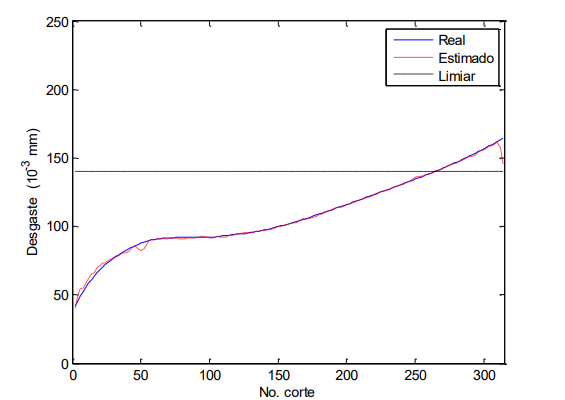
\includegraphics[scale=.4]{img/d1}}\qquad
    \subfigure[RUL da ferramenta (cutter6).]{\label{avr-datamem}%
      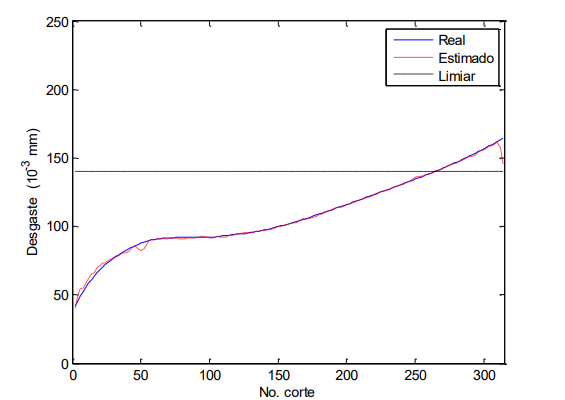
\includegraphics[scale=.4]{img/d1}}
    }
  \caption{Analise Cutter 6 \cite{inacioprognostico}}
  \label{avr-memmap}
\end{figure}
%\subsection{Tipos de Seleção de Prognósticos}

\subsection{Redes Neurais}
\subsection{Sistemas Nebulosos}
\subsection{Filtros de Partículas}

\newpage
\section{Extração de características}

Extração de características consiste em obter características especificas com base em dados observados.  O método consiste em decompor os dados já obtidos, em dados que relevantes para manter a integridade da máquina CNC, se utilizando de algoritmos \cite{liao2014discovering}.

Diversas características de domínio estatístico, frequência e tempo-frequência podem ser extraídas, desses domínios existem quatro características estatísticas mais comuns a serem extraídas e consideradas relevantes, sendo elas, Valor médio, raiz quadrada média (RMS), variância e curtose. Cada domínio pode mostrar outra visão do estado máquina \cite{wang2015enhanced}.

\begin{figure}[h]
    \centering
    %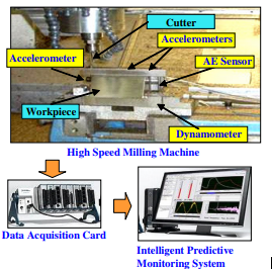
\includegraphics{img/CNC}
    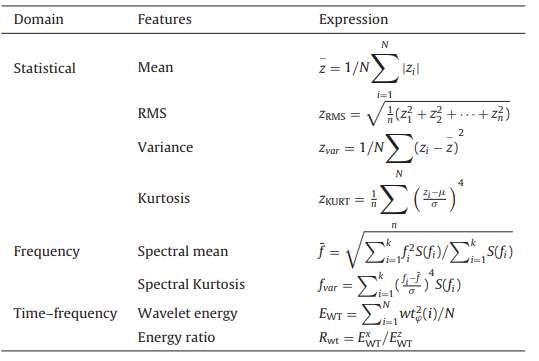
\includegraphics[scale=0.7]{img/tablect}
    \caption{Características separados por domínio \cite{wang2015enhanced} Temporario vou refazer a tabela}
\end{figure}

Em \cite{Li2009} podemos ver que a partir das características de força, foi possível se obter outras 16 caracteristicas principais usando métodos estatísticos, mostradas na Tabela 2.1.

\begin{table}[ht]
    \caption{Características Extraidas dos Sinais de Força.}
    {\centering
    \begin{tabular}{ll} \toprule
    \emph{Nº} & \emph{Característica}\\ \midrule
   1 & Erro Residual \\
2 & Diferença de primeira ordem \\
3 & Diferença de segunda ordem \\
4 & Nível Máximo de Força \\
5 & Amplitude Total da Força do Corte \\
6 & Combinação  \\
7 & mudanças de força incremental combinadas \\
8 & Desvio padrão dos componentes de força na ferramenta zona de ruptura \\
9 & Soma dos Quadrados de Erros residuais \\
10 & Taxa de pico das forças de corte \\
11 & Potência Harmônica Total \\
12 & Força Média \\
13 & Força Variável \\
14 & Desvio padrão \\
15 & Inclinação \\
16 & Curtose \\
 \bottomrule
    \end{tabular}\par
    }
\end{table}

\newpage
\section{Seleção de características}
Dado que um banco de dados, podemos ter um conjunto muito grande de dados presentes nele, muitas vezes esse conjunto possui dado que não são relevantes para o estudo a ser feito, sendo assim necessário uma seleção de tais dados. 

Após o reconhecimento dos dados presentes em tal banco de dado é feita uma extração de características, como mostrado na seção anterior. Após isso é possível que haja muitas características irrelevantes ou desnecessárias, sendo assim é necessário uma seleção de características de forma que após ela, as características selecionadas possam ser usadas para se obter o melhor resultado esperado do estudo a ser feito.

Na seleção de características, a seleção de um subconjunto de características relevantes é necessária para o estabelecer qual modelo de correlação é esperado, de forma que minimize o custo computacional \cite{Li2009}.


%\subsection{Tipos de Seleção de Características}
\subsection{Algoritmos Genéticos}
\subsection{Correlação Cruzada}
\chapter{Revisão de Literatura}

%%conceitos basicos e dps revisao

%\input{TrabalhosRelacionados}
\chapter{Metodologia}
\chapter{Desenvolvimento}

\dummytxtb\dummytxta\dummytxtc
\section{Base de dados}
\begin{figure}[ht]
    \centering
    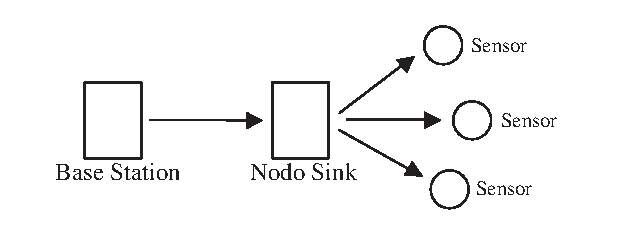
\includegraphics{img/exemplo}
    %\includegraphics[scale=.5]{exemplo-x}
    \caption{Uma figura de exemplo.}
\end{figure}

\dummytxtb

\begin{table}[ht]
    \caption{Uma tabela de exemplo.}
    {\centering
    \begin{tabular}{lcr} \toprule
    \emph{Left-aligned} & \emph{Centered} & \emph{Right-aligned} \\ \midrule
    Lorem ipsum & dolor sit & amet \\
    consectetur adipisicing & elit, sed do eiusmod & tempor \\
    incididunt ut & labore et dolore & magna aliqua. \\ \bottomrule
    \end{tabular}\par
    }
\end{table}





% \input{Resultados}
% \input{Conclusoes}

% Aqui vem a parte da bibliografia: use o comando \ppgccbibliography indicando
% apenas o nome do arquivo .bib (sem a extensão).
\ppgccbibliography{bibfile}


% Este comando encapsula o conjunto de apêndices. A sua função é fazer com que
% a numeração dos apêndices seja feita com letras maiúsculas (A, B, C, etc.) e
% a palavra "Apêndice" anteceda as entradas no Sumário.
\begin{appendices}
% Para cada apêndice, um \chapter
\chapter{Um apêndice}

\dummytxta
\dummytxtb
\dummytxtc
\dummytxta
\dummytxtb
\chapter{Outro apêndice}

\dummytxta
\dummytxtb
\dummytxtc
\dummytxta
\dummytxtb
\end{appendices} % Fim dos apêndices (usar apenas depois do último apêndice)


% Este comando encapsula o conjunto de anexos. A sua função é fazer com que a
% numeração dos anexos seja feita com letras maiúsculas (A, B, C, etc.) e a
% palavra "Anexo" anteceda as entradas no Sumário.
\begin{attachments}
% Para cada anexo, um \chapter
\chapter{Um anexo}

\dummytxta
\dummytxtb
\dummytxtc
\dummytxta
\dummytxtb
\chapter{Outro anexo}

\dummytxta
\dummytxtb
\dummytxtc
\dummytxta
\dummytxtb
\end{attachments} % Fim dos anexos (usar apenas depois do último anexo)


\end{document}
